\documentclass[border=10pt]{standalone}
\usepackage{tikz}
\begin{document}
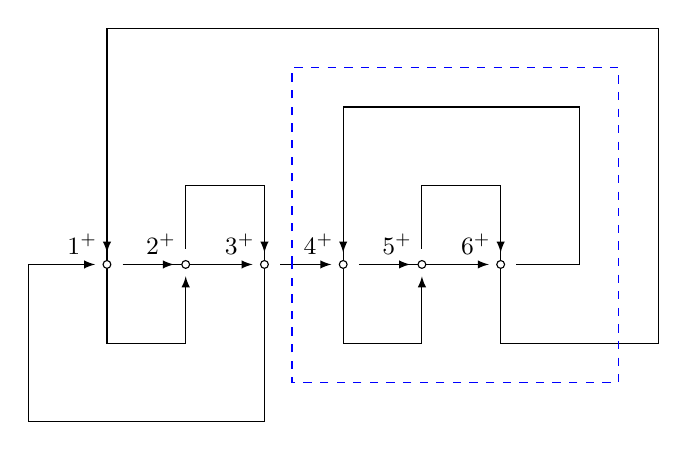
\begin{tikzpicture}
\draw[-latex](0, 0) -- (1, 0) -- (2, 0) -- (3, 0) -- (4, 0) -- (5, 0) -- (6, 0) -- (6, 2) -- (3, 2) -- (3, 0) -- (3, -1) -- (4, -1) -- (4, 0) -- (4, 1) -- (5, 1) -- (5, 0) -- (5, -1) -- (7, -1) -- (7, 0) -- (7, 3) -- (0, 3) -- (0, 0) -- (0, -1) -- (1, -1) -- (1, 0) -- (1, 1) -- (2, 1) -- (2, 0) -- (2, -2) -- (-1, -2) -- (-1, 0) -- (0, 0);
\fill[white] (-0.2, -0.2) rectangle (0.2, 0.2);
\fill[white] (0.8, -0.2) rectangle (1.2, 0.2);
\fill[white] (1.8, -0.2) rectangle (2.2, 0.2);
\fill[white] (2.8, -0.2) rectangle (3.2, 0.2);
\fill[white] (3.8, -0.2) rectangle (4.2, 0.2);
\fill[white] (4.8, -0.2) rectangle (5.2, 0.2);
\draw[-latex] (-0.8, 0) -- (-0.15000000000000002, 0);
\draw (0, 0.2) -- (0, -0.2);
\draw[-latex] (0, 1) -- (0, 0.15000000000000002);
\node[circle, fill=white, draw=black, inner sep=1pt] () at (0, 0) {};
\node[above left] () at (0, 0) {\small $1^+$};


\draw[-latex] (0.2, 0) -- (0.85, 0);
\draw (0.8, 0) -- (1.2, 0);
\draw[-latex] (1, -1) -- (1, -0.15000000000000002);
\node[circle, fill=white, draw=black, inner sep=1pt] () at (1, 0) {};
\node[above left] () at (1, 0) {\small $2^+$};


\draw[-latex] (1.2, 0) -- (1.85, 0);
\draw (2, 0.2) -- (2, -0.2);
\draw[-latex] (2, 1) -- (2, 0.15000000000000002);
\node[circle, fill=white, draw=black, inner sep=1pt] () at (2, 0) {};
\node[above left] () at (2, 0) {\small $3^+$};


\draw[-latex] (2.2, 0) -- (2.85, 0);
\draw (3, 0.2) -- (3, -0.2);
\draw[-latex] (3, 1) -- (3, 0.15000000000000002);
\node[circle, fill=white, draw=black, inner sep=1pt] () at (3, 0) {};
\node[above left] () at (3, 0) {\small $4^+$};


\draw[-latex] (3.2, 0) -- (3.85, 0);
\draw (3.8, 0) -- (4.2, 0);
\draw[-latex] (4, -1) -- (4, -0.15000000000000002);
\node[circle, fill=white, draw=black, inner sep=1pt] () at (4, 0) {};
\node[above left] () at (4, 0) {\small $5^+$};


\draw[-latex] (4.2, 0) -- (4.85, 0);
\draw (5, 0.2) -- (5, -0.2);
\draw[-latex] (5, 1) -- (5, 0.15000000000000002);
\node[circle, fill=white, draw=black, inner sep=1pt] () at (5, 0) {};
\node[above left] () at (5, 0) {\small $6^+$};

\draw[dashed, blue] (2.35, 0) -- (2.35, 2.5) -- (6.5, 2.5) -- (6.5,
-1.5) -- (2.35, -1.5) -- (2.35, 0);

\end{tikzpicture}
\end{document}
